\chapter{Sistema Proposto}\label{cap3}

Essa seção apresenta as etapas de desenvolvimento do sistema de recuperação de atas proposto, bem como o seu funcionamento geral, desde a preparação dos documentos até a entrega dos históricos de ocorrência ao usuário. O sistema proposto tem como objetivo permitir ao usuário consultar uma coleção de documentos de reuniões a fim de obter todo o histórico de ocorrências de um determinado tema relacionado à pesquisa do usuário, podendo identificar nos documentos onde esse tema foi mencionado, bem como se houve uma decisão sobre o tema. Para isso, o sistema é divido em dois módulos principais: módulo de preparação e manutenção e módulo de consulta, os quais serão detalhados nas próximas seções.  % "isso envolve a classificação. Onde entram os tópicos?" --> Rafael


  %--- Figura Visão Geral ---
  \begin{figure}[!h]
	  \centering
	  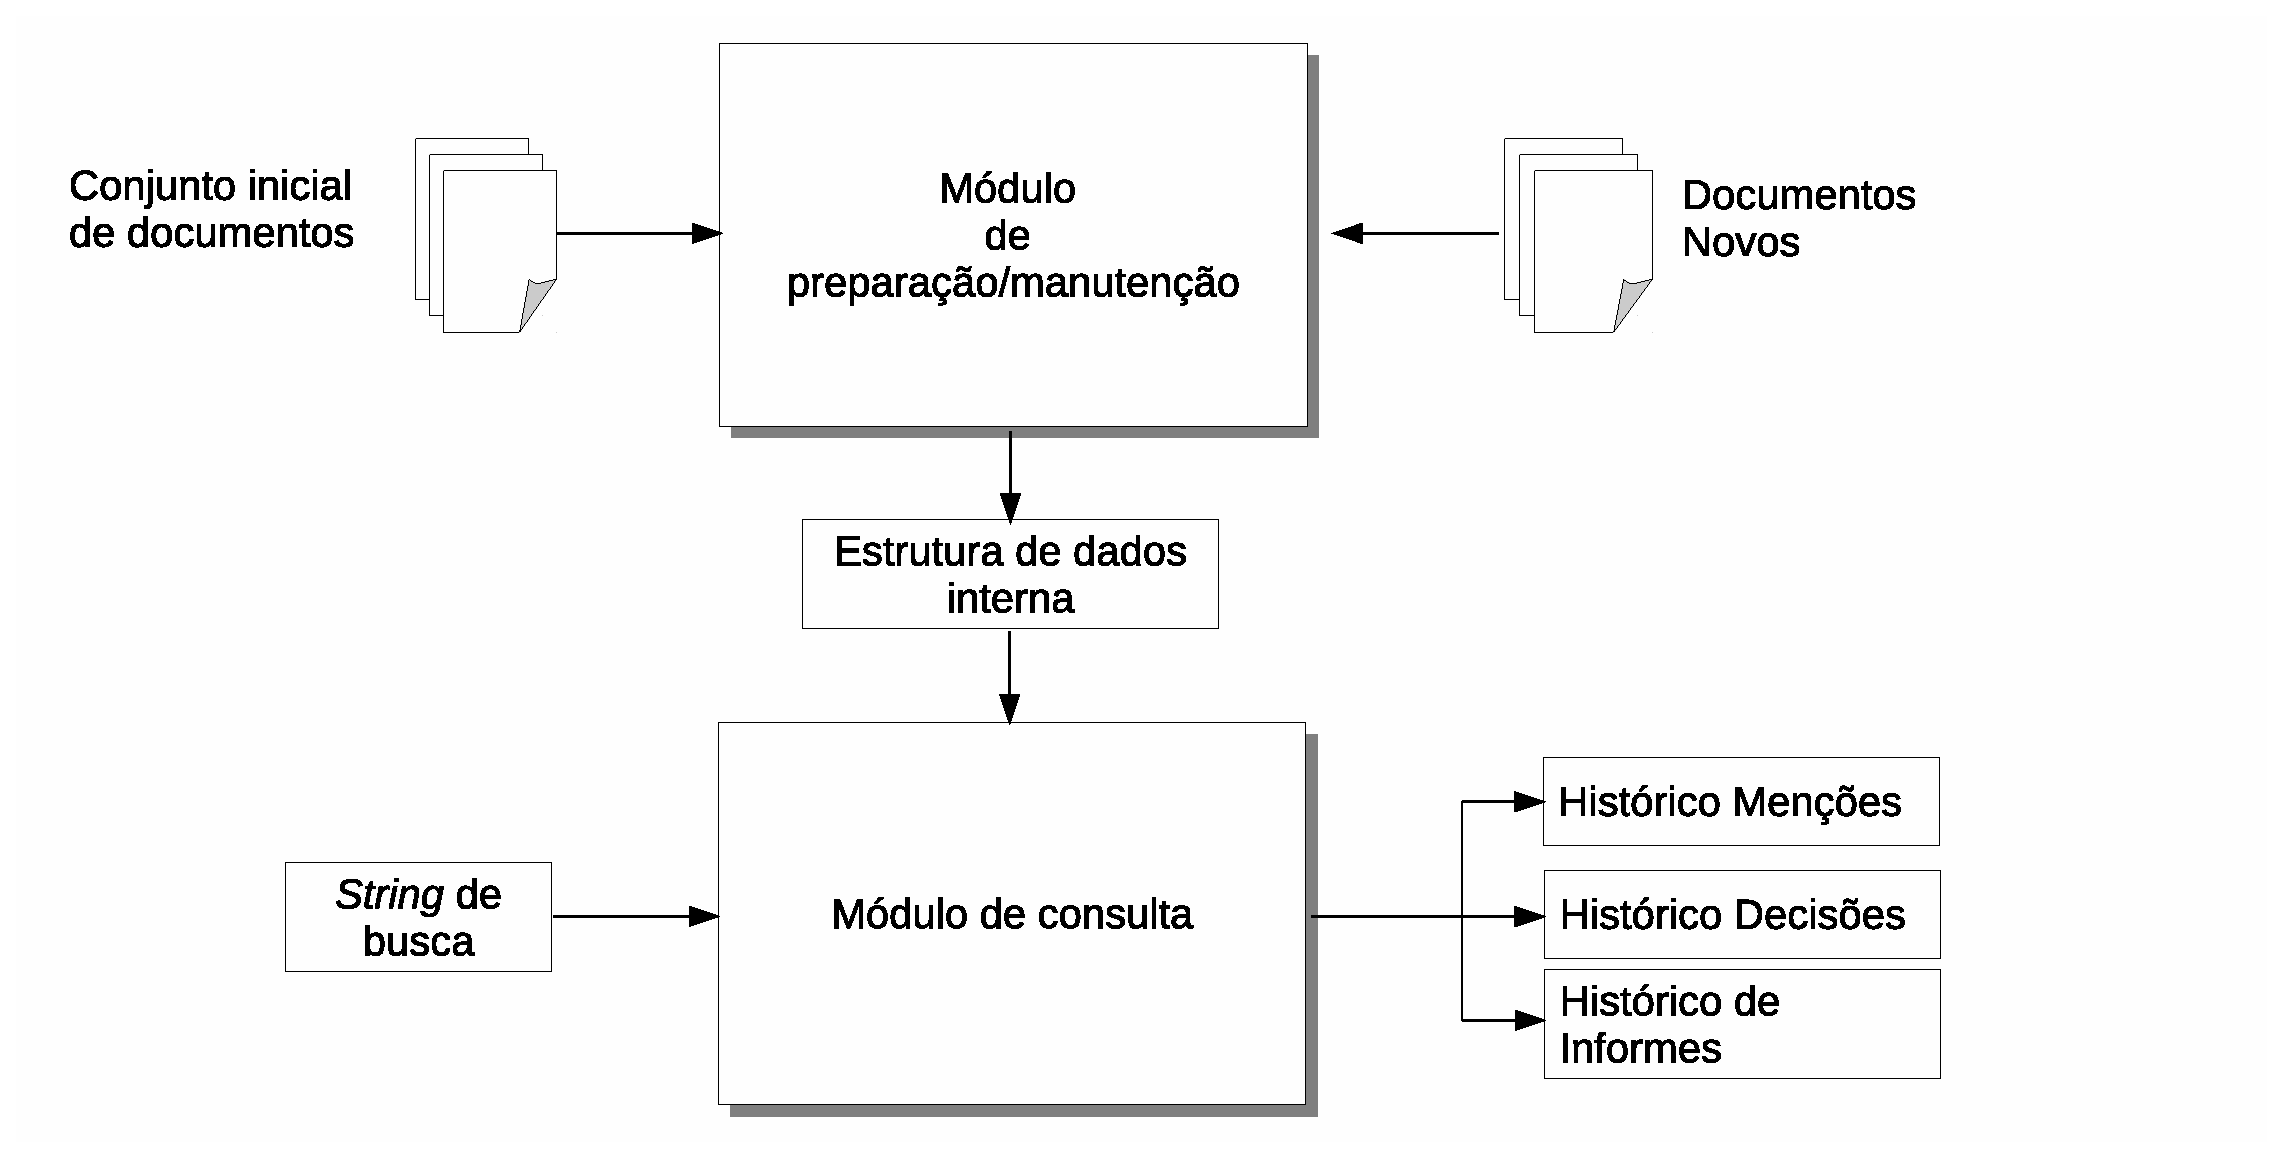
\includegraphics[width=0.69\paperwidth]{conteudo/capitulos/figs/visao-geral-3.eps}
	  \caption{Visão geral do sistema}
	  \label{fig:visao-geral}
  \end{figure}

A Figura \ref{fig:visao-geral} mostra a visão geral do sistema com suas principais entradas e saídas. Inicialmente o sistema recebe um conjunto inicial de documentos. A função de Módulo de preparação/manutenção é processar e manter esses textos para gerar uma base de dados interna que codifica os textos extraídos com seus respetivos tópicos. O Módulo de consulta recebe a consulta do usuário que expressa o assunto de interesse. Em seguida, os trechos de texto que fazem menção ao esse assunto são exibidos ao usuário.




A proposta original deste trabalho contempla funcionalidades de classificação para identificar automaticamente, contudo essas funcionalidades configuram trabalhos futuros para continuação do sistema como concebido inicialmente. Assim, está focada na segmentação de atas de reunião, no agrupamento desses segmentos em tópicos e na recuperação de trechos de atas relacionados ao assunto da pesquisa.




% ========== Módulo de Preparação e manutenção ==========

\section{Módulo de preparação e manutenção}\label{sec:modulo-preparacao}


O módulo de preparação e manutenção tem como função principal manter uma base de dados necessária para os processos de recuperação de informação. Inicialmente, esse módulo deve receber um conjunto inicial de documentos os quais devem ser divididos em segmentos de texto que contêm um assunto predominante, e agrupá-los em categorias por meio de técnicas de extração de tópicos. Além disso, considera-se o crescimento da bases de documentos, assim, o sistema deve receber novos documentos a medida que são gerados. 








% melhorar ↓↓↓↓↓
% A seguir são apresentadas as etapas do módulo de preparação e manutenção desde a preparação dos documentos até a entrega da estrutura interna ao módulo de consulta. 

% Inicialmente serão descritos a seleção e pré-processamento das atas. 



% ==================== O Corpus ===================== %



% ========== Preparação dos Documentos ==========

\subsection{Preparação dos documentos}


As atas são normalmente armazenadas em arquivos binários do tipo \textit{pdf}, \textit{doc}, \textit{docx} ou \textit{odt}. As atas devem ser pré-processadas e estruturadas para que possam ser aplicados métodos de MI e RI. Inicialmente, o texto puro é extraído e passa por processos de transformação que incluem remoção de elementos considerados menos significativos e a identificação de sentenças. Esse processo é ilustrado na Figura~\ref{fig:preprocessamento-segmentacao} e descrito a seguir.

\begin{center}
	\begin{figure}[h!]

		% 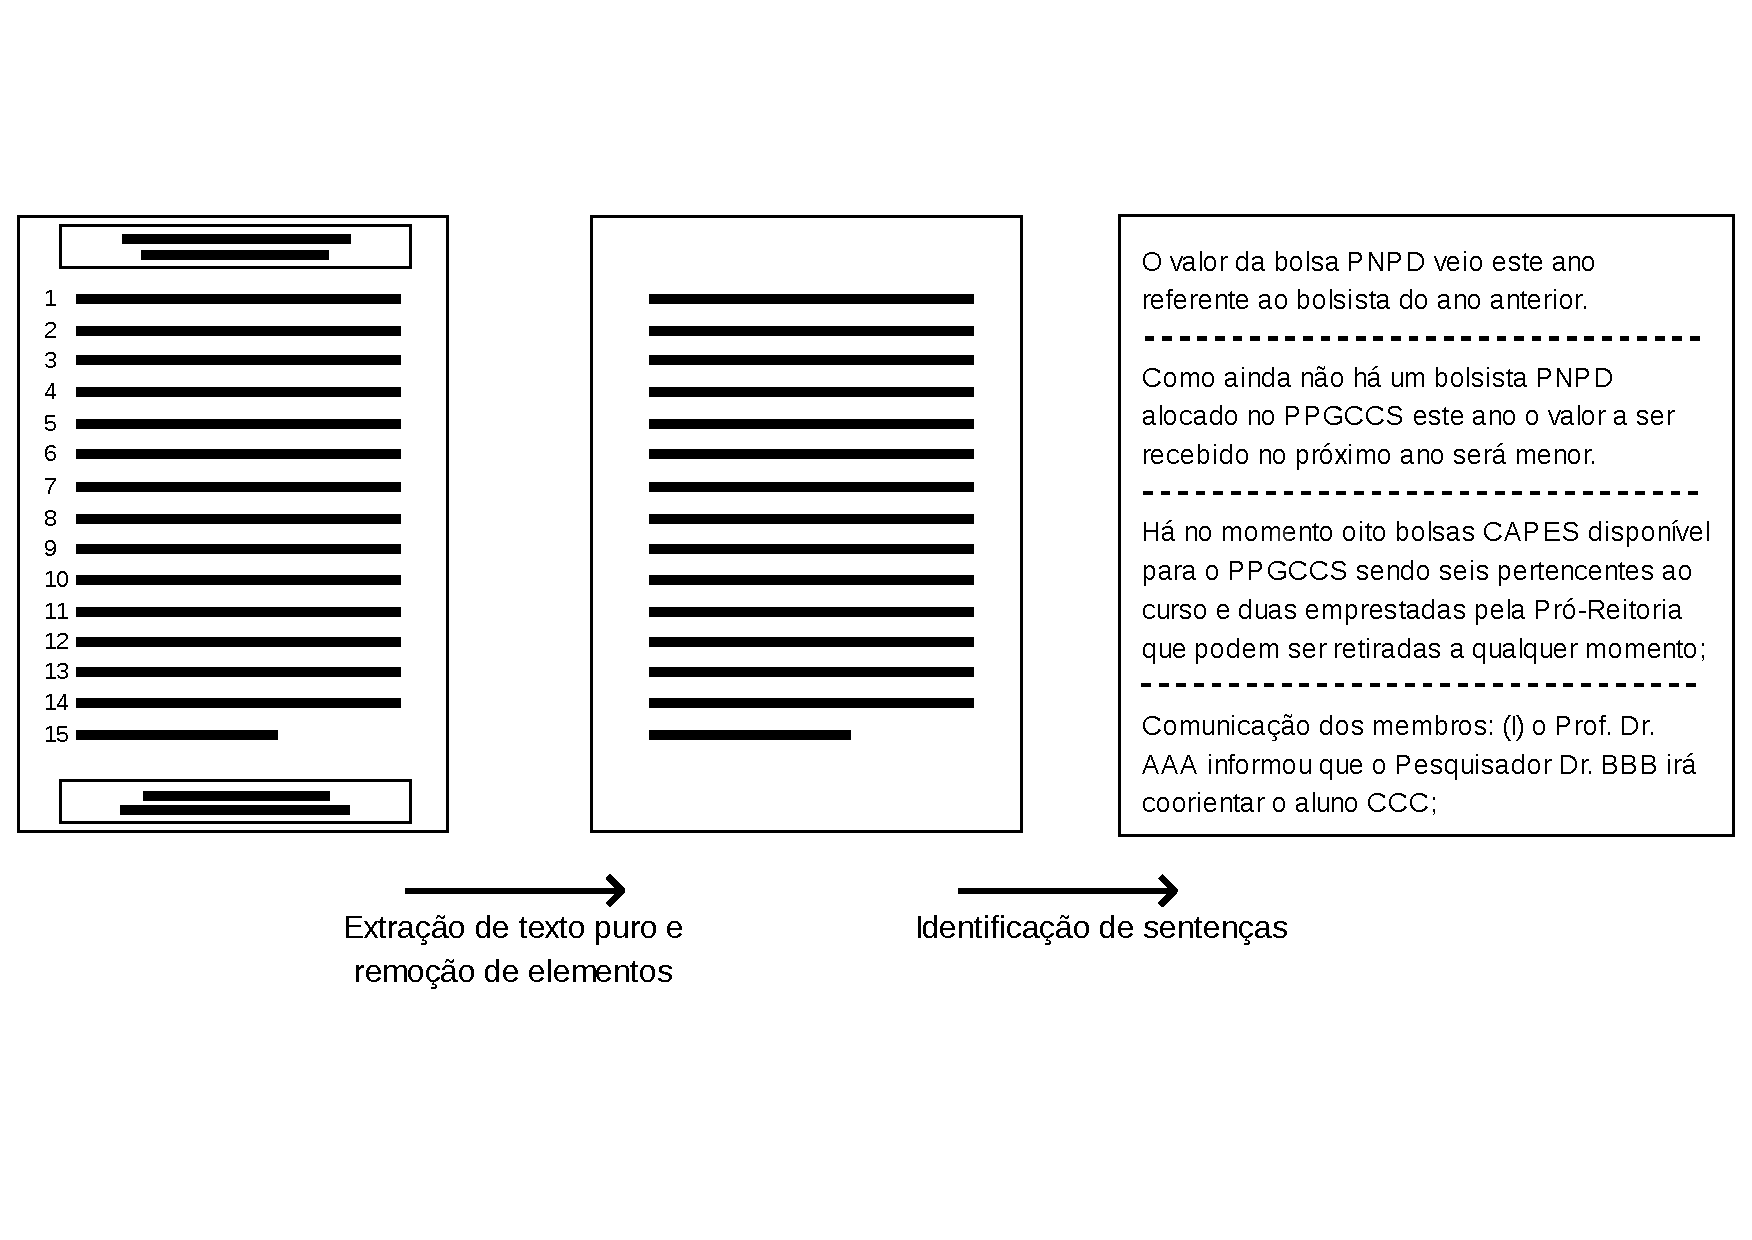
\includegraphics[trim={ 0 140 0 140 },clip,page=1,width=\textwidth]{conteudo/capitulos/figs/preparacao-docs.pdf}
		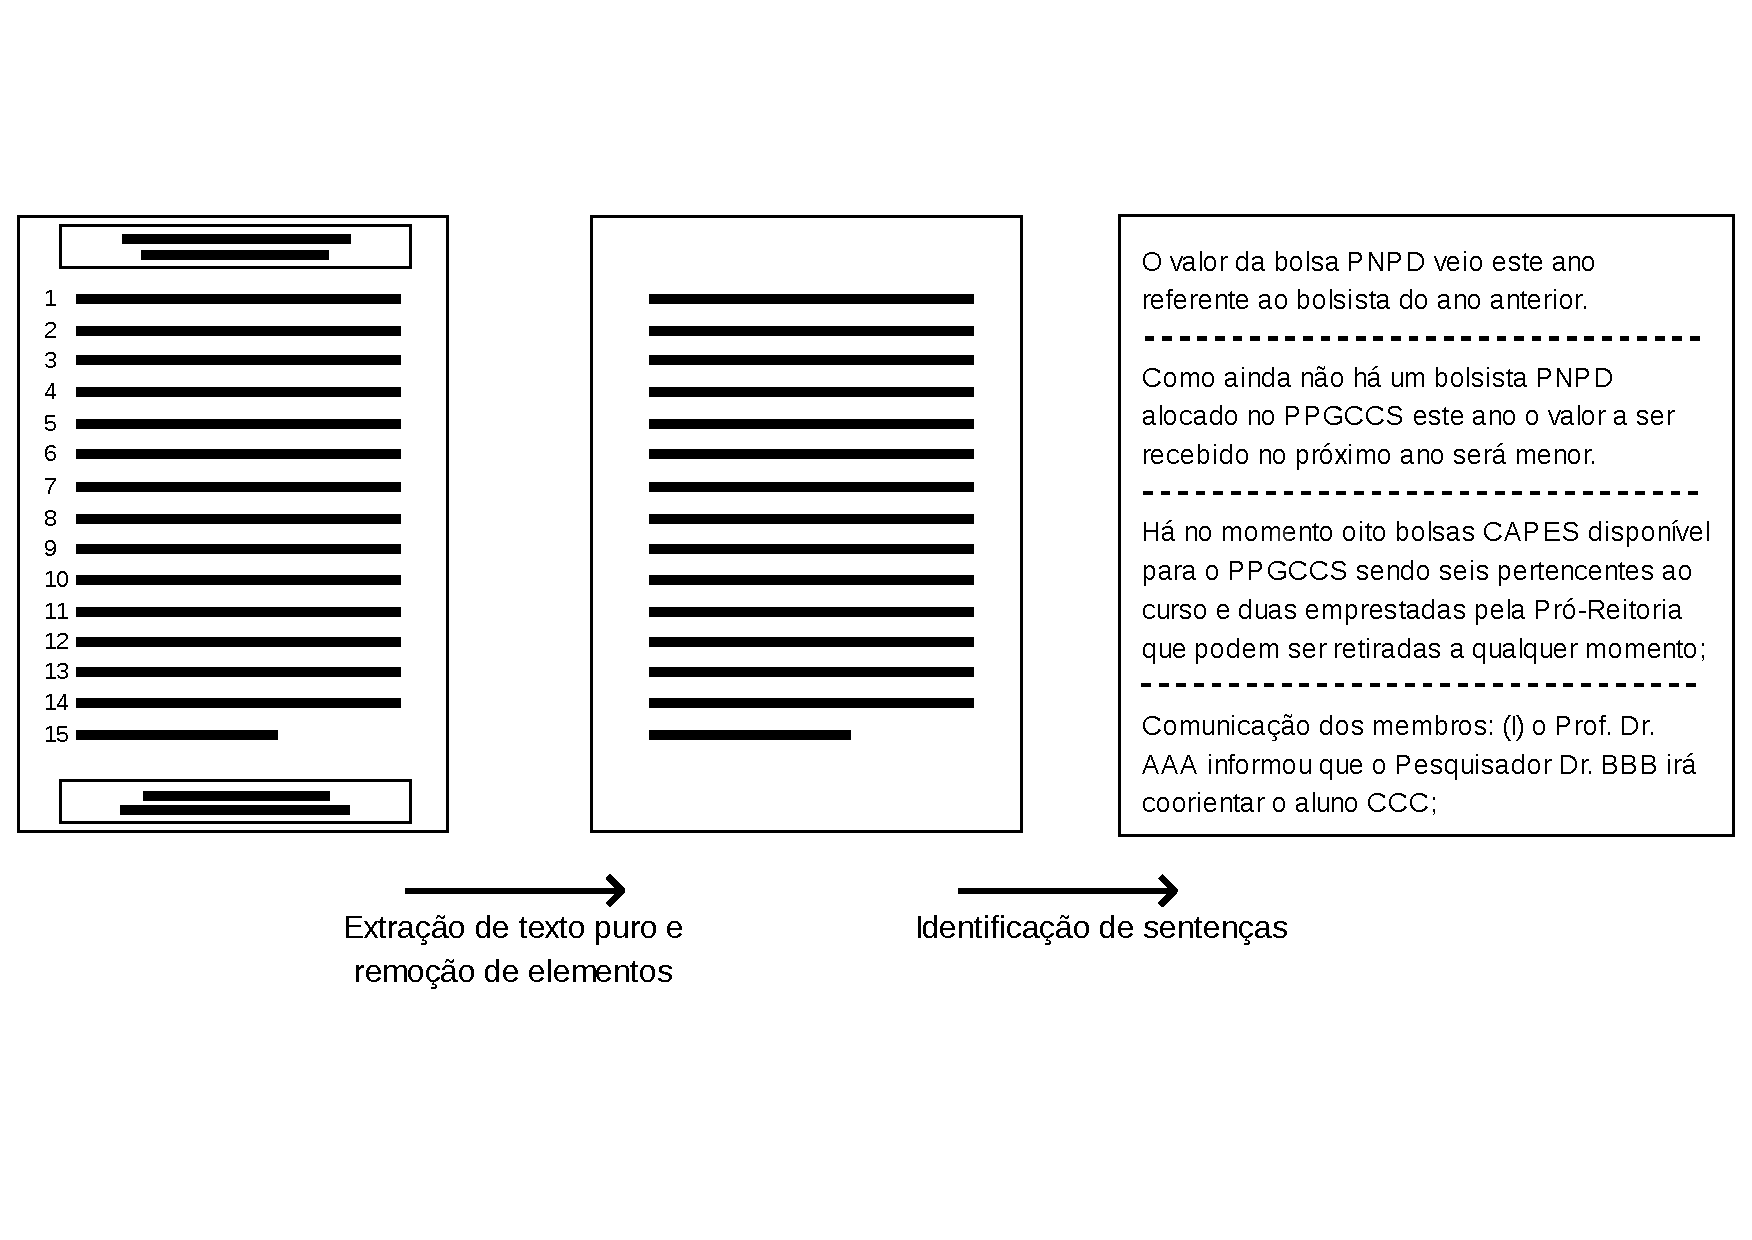
\includegraphics[trim={ 0 100 0 100 },clip,page=1,width=\textwidth]{conteudo/capitulos/figs/preparacao-docs.pdf}

		\caption{Etapa de preparação de um documento que inclui da extração de texto puro,  remoção de elementos menos significativos e a identificação de sentenças}
		\label{fig:preprocessamento-segmentacao}
	\end{figure}
\end{center}


% -> Essa imagem deve ser mais completa. desde a extração dos textos até os subdocumentos;


%  Cabeçalhos e rodapés
% Remoção de cabeçalhos: 
As atas contém trechos que podem ser considerados pouco informativos e descartados durante o pré-processamento, como cabeçalhos e rodapés que se misturam aos tópicos tratados na reunião, podendo ser inseridos no meio de um tópico prejudicando tanto os algoritmos de MT e RI, quanto a leitura do texto pelo usuário. Um cabeçalho é a porção de texto que inicia cada página do documento e, de forma semelhante, um rodapé e a porção que as encerra. Detecta-se os cabeçalhos e os rodapés sempre que há uma repetição das primeiras e últimas palavras do documento.


%  Identificação de sentenças
% \item 
% Identificação sentenças: 
Nesse trabalho considera-se as sentenças as menores unidades de informação a serem processadas pelos algoritmos de segmentação, por tanto, devem ser identificadas. Ao considerar intuitivamente que uma sentença seja uma sequência de palavras entre sinais de pontuação como ``.'', ``!'' e ``?'', alguns erros poderiam ocorrer quando esses tiverem outra função dentro do texto como em abreviações\footnote{As abreviações são identificadas por meio de uma lista com 234 abreviações conhecidas.}, endereços de internet e datas. Outro problema seriam frases curtas com poucas palavras e que não expressam um conceito completo, mas parte dele. Devido ao estilo de pontuação desses documentos, como encerrar sentenças usando um ``;'' e inserção de linhas extras, foram usadas as regras especiais para identificação de finais de sentença. No Algoritmo~\ref{alg:identificacaofinaisdesent} é mostrado como cada \textit{token} é identificado e como final de sentença.  % Os detalhes sobre essas regras estão disponíveis para consulta em \urlsoftwares.


\begin{algorithm}
	\SetKwInOut{Input}{Entrada}
	\SetKwInOut{Output}{Saída}
	\SetKwBlock{Inicio}{início}{fim}
	\SetKwFor{ParaTodo}{para todo}{}{fim para todo}
	\SetKwIF{Se}{SenaoSe}{Senao}{}{}{senao se}{senao}{fim se}
	\SetKwFor{Para}{}{}{}
%	\SetKwAlgorithm{Algorithm}{Algoritmo}{}

	
	\Input{Texto}
	\Output{Texto com identificações de finais de sentença}
	
	\ParaTodo {token, marcá-lo como final de sentença se:} {	

	Terminar com um \texttt{!}\\
	Terminar com um \texttt{.} e não for uma abreviação\\
	Terminar em \texttt{.?;} e:
		\Para{}{
			For seguido de uma quebra de parágrafo ou tabulação\\
			O próximo \textit{token} iniciar com  \texttt{(\{["'}\\
			O próximo \textit{token} iniciar com letra maiúscula\\
			O penúltimo caracter  for \texttt{)\}]"'}\\
		}
	}
	
	\caption{Identificação de finais de sentença.}
	\label{alg:identificacaofinaisdesent}
\end{algorithm}

% \end{enumerate}
	



% ========== Pré-Processamento dos Documentos ==========


\subsection{Pré-Processamento dos Documentos}


Na etapa de pré-processamento, os documentos são pré-processados individualmente conforme são recebidos pelos algoritmos de segmentação extração de tópicos. Inicialmente, cada texto passou por um processo de transformação em que as letras foram convertidas em caixa baixa e eliminou-se sinais de pontuação, numerais e termos menores que três caracteres. Em seguida removeu-se os termos que não contribuem para a etapa de segmentação, as quais são chamadas de \textit{stop words}, para identificá-las usou-se uma lista de 438 palavras. Em seguida, extraiu-se o radical de cada palavra por meio da técnica \textit{stemming}. 

Nesse trabalho, todos os termos restantes após a remoção de \textit{stop words} e \textit{stemming} foram mantidas independentemente de valores de   \textit{Document Frequency} devido a característica das atas de possuir múltiplos assuntos em um documento que posteriormente serão considerados sub-documentos relativamente independentes os quais contém em média 70 termos. 




% Uma imagem para o pré-processamento


% Uma tabela com as modificações

		% Documento | Total de Termos | Termos removidos | Termos com DF >= 2










% ==================== Segmentação ===================== %

\subsection{Segmentação}

Como já mencionado, uma ata registra a sucessão de assuntos discutidos em uma reunião, porém apresenta-se com poucas quebras de parágrafo e sem marcações de estrutura, como capítulos, seções ou quaisquer indicações sobre o assunto do texto. Portanto, faz-se necessário descobrir quando há uma mudança de assunto no texto da ata. Para essa tarefa, as técnicas de segmentação de texto recebem uma lista de sentenças, da qual considera cada ponto entre duas sentenças como candidato a limite, ou seja, um ponto onde há transição entre assuntos~\cite{Bokaei2015, Bokaei2016, Misra2009, Sakahara2014}.

As técnicas de segmentação aboradas na Subseção~\ref{sec:segmentacao} divdiem o texto de cada ata em trechos que contêm um assunto relativamente independente, aqui chamdaos de sub-documentos. Esses sub-documentos serão processados por um extrator de tópicos que irá extrair descritores e agrupalos por tópicos.





% ==================== Extração de Tópicos ===================== %

\subsection{Extração de Tópicos}

O resultado do processo de extração de tópicos é a representação dos documentos e seus tópicos em uma matriz documento-tópico que atribui um peso a cada tópico para cada documento e uma matriz termo-tópico que pode representar a probabilidade de ocorrência do termo quando um tópico ocorre em documento ou a frequência esperada desse termo.  
Nesse sistema, essas representações são utilizadas para melhorar as tarefas de recuperação de informação e agrupamento dos documentos. 
O agrupamento por tópicos e seus descritores são utilizados para ajudar o usuário a analisar e identificar os subdocumentos conforme sua consulta, bem como encontrar resultados similares.


% --> explicar o que são descritores;
% os descritores são utilizados;


% ==================== Estrutura de Dados Interna ===================== %

\subsection{Estrutura de Dados Interna}

A estrutura de dados interna é o resultado dos processos de segmentação e extração de tópicos. Constituída por: 
(1) documentos originais para referência, 
(2) segmentos de texto contendo um assunto relativamente independente,
(3) matrizes documento-tópico e termo-tópico.
Na Figura~\ref{fig:estrutura-dados-interna} é apresentado a visão geral da estrutura de dados interna. 


% deve ser atualizada a cada novo documento inserido no sistema.



	\begin{figure}[h!]
\center
		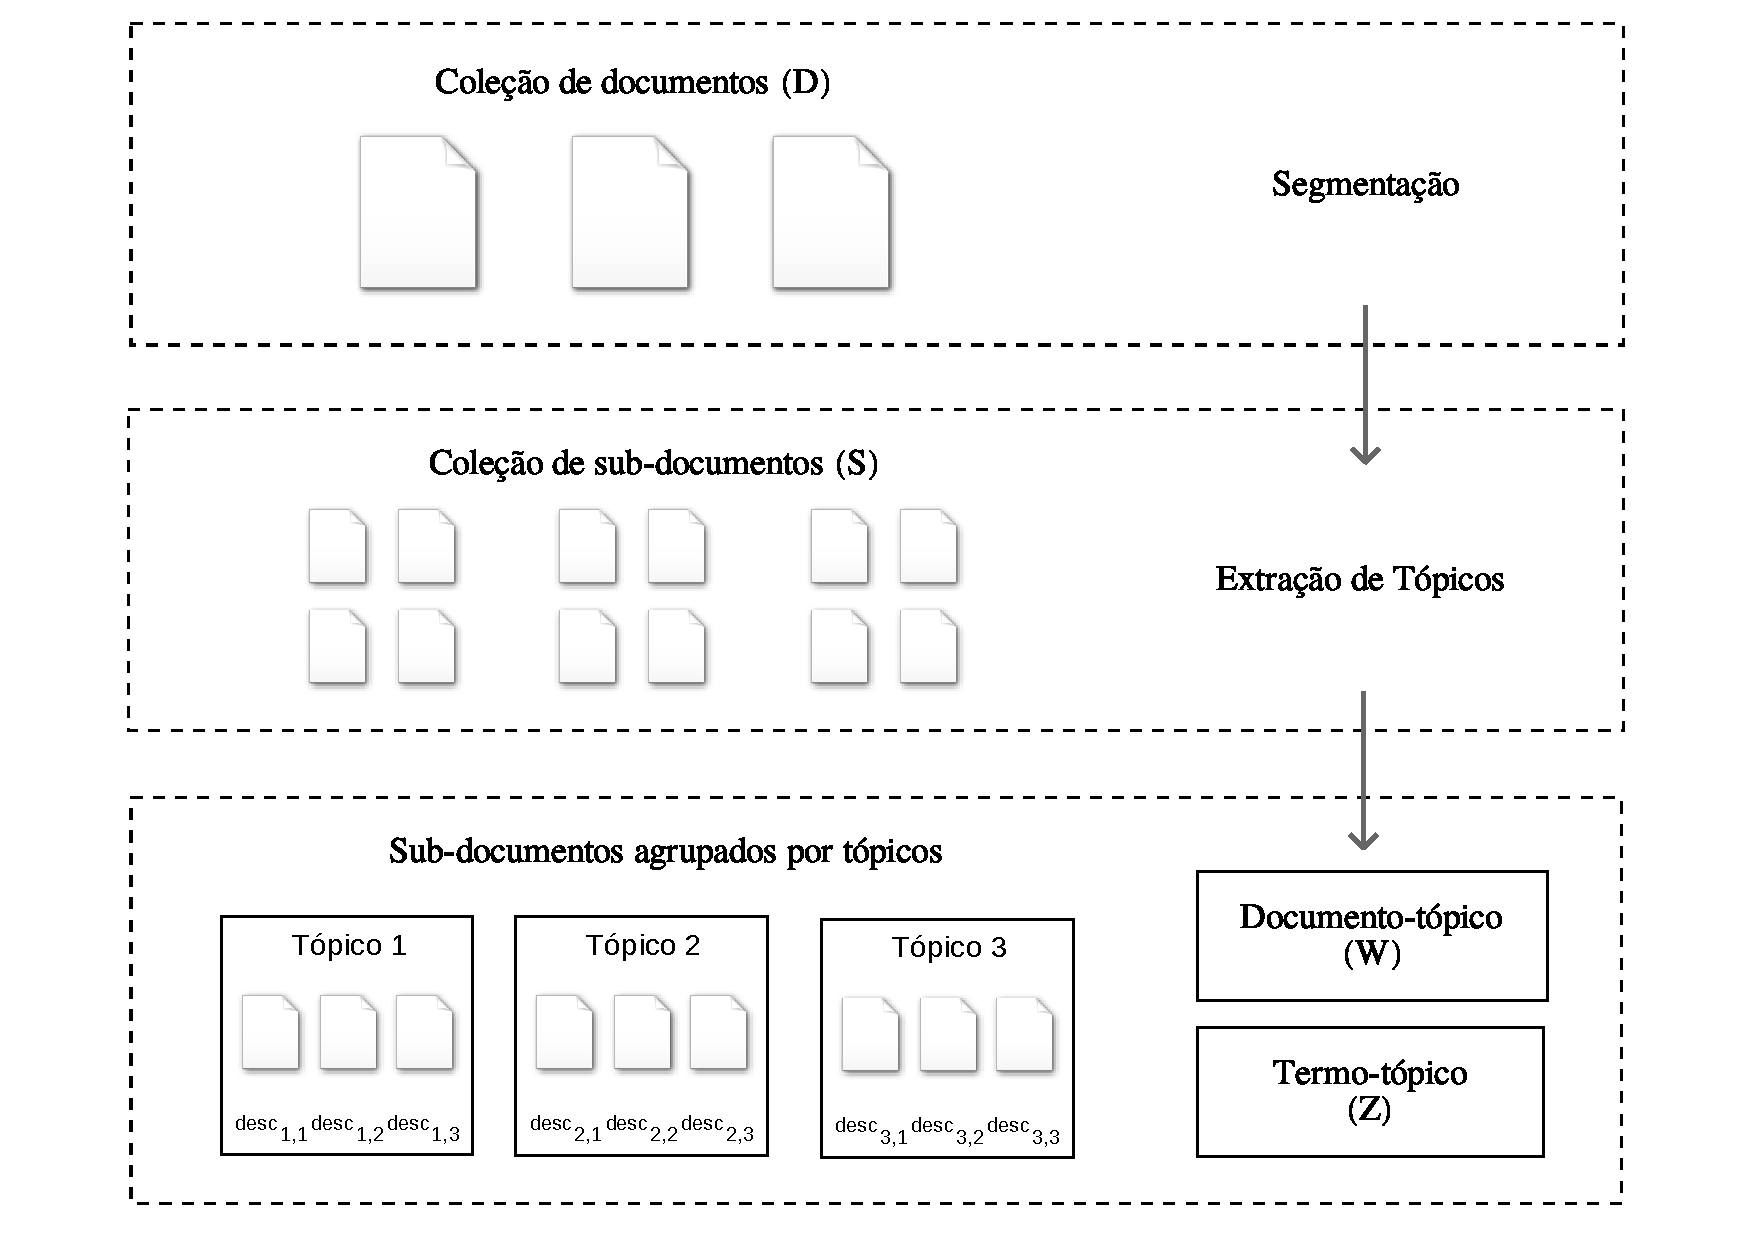
\includegraphics[trim={ 61 0 61 0 },clip,page=1,width=0.9\textwidth]{conteudo/capitulos/figs/estrutura-de-dados-interna.pdf}

		\caption{Visão geral da estrutura de dados interna e seu processo de geração.}
		\label{fig:estrutura-dados-interna}
	\end{figure}




Os arquivos da coleção de documentos $(D)$ são mantidos para reverência aos textos integrais fincando disponíveis para visualização e fonte original das informações.  
Os segmentos de textos $(S)$ gerados pela segmentação dos documentos originais $(D)$ são armazenadas em arquivos de texto plano que são tratados como sub-documentos pelo sistema os quais contém os textos a serem exibidos ao usuário pelo módulo de consulta.  
É a partir desses sub-documentos que o extrator de tópicos constrói as matrizes documento-tópico e termo-tópico. Uma vez construídas, essas matrizes são armazenadas em arquivos e usadas para identificar os melhores descritores para cada tópicos bem como o agrupamento dos sub-documentos.








% ==================== Módulo de Consulta ===================== %

\section{Módulo de Consulta}


Uma vez que a estrutura de dados interna contem os assuntos abordados na coleção de documentos, o tipo de ocorrência para cada assunto e o trecho onde se encontram, 
é responsabilidade do módulo de consulta receber a \textit{string} de consulta do usuário, resgatar os dados desejados e apresentá-los em ordem cronológica, dando condições para o usuário acessar os segmentos encontrados bem como os documentos originais.

% \subsection{Seleção dos tópicos}

\subsection{Visualização}

O usuário final precisa de uma interface adequada para visualizar os resultados da busca considerando-se a relevância dos tópicos selecionados e a sequência cronológica. Uma boa apresentação deve permitir ao usuário identificar a relevância os resultados e ser relativante independente para compreensão do conteúdo, evitando a leitura do texto completo. Ou seja, o texto de cada tópico apresentado deve ser suficiente para compreensão do assunto mencionado, sem necessidade de visualizar o documento original.

As informações apresentadas, incluem dados obtidos do documento como o nome do arquivo, e o texto onde o assunto é mencionado. Além disso, apresenta-se as informação extraídas pelas técnicas de mineração de texto como os descritores e rótulos. Para cada busca, é retornada uma lista de resultados ordenados pela relevância com a \textit{string} de entrada, sendo cada item referente a uma menção a um assunto. Um tópico é abordado em diferentes momentos e registrado em atas distintas, onde cada menção é um resultado a ser apresentado. 

Como parte da proposta, o sistema apresenta cada resultado dentro de um histórico de menções. Para isso, abaixo do texto é exibida uma linha com links para os resultados que compartilham o mesmo tópico ordenados por data. Os links, ao ser acionado, direciona para o resultado que aponta, além disso, quando o cursor do mouse está sobre o link, é apresentado um pre-visualização do texto. Dessa forma o usuário tem acesso uma interface que lhe fornece uma visão temporal das menções.


% Uma vez que um item faz menção a um tópico específico, 
% o sistema traz vários resultados para uma consulta, alguns mais relevantes que outros. Para cada resultado (que podem tratar de coisas diferentes) o sistema apresenta um histórico de menções para aquele assunto;


% \section{Estudo de caso}
% -- qual o ganho em relação a um sitema de busca por palavras-chave? 

















